\documentclass{article}\usepackage[]{graphicx}\usepackage[]{xcolor}
% maxwidth is the original width if it is less than linewidth
% otherwise use linewidth (to make sure the graphics do not exceed the margin)
\makeatletter
\def\maxwidth{ %
  \ifdim\Gin@nat@width>\linewidth
    \linewidth
  \else
    \Gin@nat@width
  \fi
}
\makeatother

\definecolor{fgcolor}{rgb}{0.345, 0.345, 0.345}
\newcommand{\hlnum}[1]{\textcolor[rgb]{0.686,0.059,0.569}{#1}}%
\newcommand{\hlsng}[1]{\textcolor[rgb]{0.192,0.494,0.8}{#1}}%
\newcommand{\hlcom}[1]{\textcolor[rgb]{0.678,0.584,0.686}{\textit{#1}}}%
\newcommand{\hlopt}[1]{\textcolor[rgb]{0,0,0}{#1}}%
\newcommand{\hldef}[1]{\textcolor[rgb]{0.345,0.345,0.345}{#1}}%
\newcommand{\hlkwa}[1]{\textcolor[rgb]{0.161,0.373,0.58}{\textbf{#1}}}%
\newcommand{\hlkwb}[1]{\textcolor[rgb]{0.69,0.353,0.396}{#1}}%
\newcommand{\hlkwc}[1]{\textcolor[rgb]{0.333,0.667,0.333}{#1}}%
\newcommand{\hlkwd}[1]{\textcolor[rgb]{0.737,0.353,0.396}{\textbf{#1}}}%
\let\hlipl\hlkwb

\usepackage{framed}
\makeatletter
\newenvironment{kframe}{%
 \def\at@end@of@kframe{}%
 \ifinner\ifhmode%
  \def\at@end@of@kframe{\end{minipage}}%
  \begin{minipage}{\columnwidth}%
 \fi\fi%
 \def\FrameCommand##1{\hskip\@totalleftmargin \hskip-\fboxsep
 \colorbox{shadecolor}{##1}\hskip-\fboxsep
     % There is no \\@totalrightmargin, so:
     \hskip-\linewidth \hskip-\@totalleftmargin \hskip\columnwidth}%
 \MakeFramed {\advance\hsize-\width
   \@totalleftmargin\z@ \linewidth\hsize
   \@setminipage}}%
 {\par\unskip\endMakeFramed%
 \at@end@of@kframe}
\makeatother

\definecolor{shadecolor}{rgb}{.97, .97, .97}
\definecolor{messagecolor}{rgb}{0, 0, 0}
\definecolor{warningcolor}{rgb}{1, 0, 1}
\definecolor{errorcolor}{rgb}{1, 0, 0}
\newenvironment{knitrout}{}{} % an empty environment to be redefined in TeX

\usepackage{alltt}
\usepackage{amsmath} %This allows me to use the align functionality.
                     %If you find yourself trying to replicate
                     %something you found online, ensure you're
                     %loading the necessary packages!
\usepackage{amsfonts}%Math font
\usepackage{graphicx}%For including graphics
\usepackage{hyperref}%For Hyperlinks
\usepackage[shortlabels]{enumitem}% For enumerated lists with labels specified
                                  % We had to run tlmgr_install("enumitem") in R
\hypersetup{colorlinks = true,citecolor=black} %set citations to have black (not green) color
\usepackage{natbib}        %For the bibliography
\setlength{\bibsep}{0pt plus 0.3ex}
\bibliographystyle{apalike}%For the bibliography
\usepackage[margin=0.50in]{geometry}
\usepackage{float}
\usepackage{multicol}

%fix for figures
\usepackage{caption}
\newenvironment{Figure}
  {\par\medskip\noindent\minipage{\linewidth}}
  {\endminipage\par\medskip}
\IfFileExists{upquote.sty}{\usepackage{upquote}}{}
\begin{document}

\vspace{-1in}
\title{Lab 7 and 8 -- MATH 240 -- Computational Statistics}

\author{
  Camilo Granada Cossio \\
  Colgate University  \\
  Mathematics Department  \\
  {\tt cgranadacossio@colgate.edu}
}

\date{}

\maketitle

\begin{multicols}{2}
\begin{abstract}
This lab explored the statistical properties and applications of the Beta distribution using \texttt{R}. Derivations and simulations were conducted to describe the shape, behavior, and use cases of the distribution. Using \texttt{tidyverse} \citep{tidyverse} and \texttt{cumstats} \citep{cumstat}, key properties such as mean, variance, skewness, and kurtosis were derived and compared to sdample-based summaries. Parameter estimates were generated using the Method of Moments and Maximum Likelihood Estimation. These estimation methods were evaluated through simulations and applied to global death rate data from the World Bank (2022).
\end{abstract}

\noindent \textbf{Keywords:} Beta distribution; Parameter estimation; Simulation; Method of Moments; Maximum Likelihood Estimation

\section{Introduction}

\indent The Beta distribution is a flexible model for continuous variables bounded between 0 and 1, often used for proportions, probabilities, and rates. It is defined by two shape parameters $\alpha$ and $\beta$, which determine the distributions form. Depending on these parameters, the distribution can appear left-skewed, right-skewed, symetric, or U-shaped.

Building on this, this lab investigates the Beta distribution by deriving its key statistics using closed-form expressions for the mean, variance, skewness, and excess kurtosis. These statistics are explored under different parameter values to understand how $\alpha$ and $\beta$ influence distribution behavior. The lab also examines how sample-based summaries compare to population characteristics and evaluates the Method of Moments and Maximum Likelihood Estimation through simulations and real-world data.

\section{Density Functions and Parameters}

The probability density function (PDF) of the Beta distributions is:
\begin{equation*}
f(x|\alpha, \beta) = \frac{\Gamma(\alpha + \beta)}{\Gamma(\alpha)\Gamma(\beta)} x^{\alpha - 1}(1 - x)^{\beta - 1} \quad \text{for } x \in [0, 1],
\end{equation*}
where $\alpha, \beta > 0$ and $\Gamma(\cdot)$ is the gamma function.

The shape of the distribution is fully determined by $\alpha$ and $\beta$. The following examples illustrate its flexibility: 
\begin{itemize}
\item Beta(2, 5): Right-skewed
\item Beta(5, 5): Symmetric
\item Beta(5, 2): Left-skewed
\item Beta(0.5, 0.5): U-shaped
\end{itemize}


\section{Properties}

Several population-level characteristics of the Beta distribution are derived from its PDF:
\begin{align*}
\text{Mean: } & \mathbb{E}(X) = \frac{\alpha}{\alpha + \beta} \\
\text{Variance: } & \text{Var}(X) = \frac{\alpha \beta}{(\alpha + \beta)^2 (\alpha + \beta + 1)} \\
\text{Skewness: } & \frac{2(\beta - \alpha) \sqrt{\alpha + \beta + 1}}{(\alpha + \beta + 2) \sqrt{\alpha \beta}} \\
\text{Excess Kurtosis: } & \frac{6[(\alpha - \beta)^2 (\alpha + \beta + 1) - \alpha \beta (\alpha + \beta + 2)]}{\alpha \beta (\alpha + \beta + 2)(\alpha + \beta + 3)}
\end{align*}
These theoretical values were compared to those computed using \texttt{R} functions for each formula. The \texttt{cumstats} and \texttt{tidyverse} packages were used to summarize the behavior of these statistics from samples.

\section{Estimators}

To estimate $\alpha$ and $\beta$ from the data, two approaches were used: 
\begin{itemize}
\item \textbf{Method of Moments (MOM):} Matches sample moments to theoretical moments
\item \textbf{Maximum Likelihood Estimation (MLE):} Optimizes the log-likelihood based on the PDF.
\end{itemize}
Simulations with $n = 1000$ showed that MLE offers improved performance over MOM, including higher precision and lower error. The quality of the estimators was assessed using:
\begin{align*}
\text{Bias: } & \mathbb{E}(\hat{\theta}) - \theta \\
\text{Precision: } & \frac{1}{\text{Var}(\hat{\theta})} \\
\text{MSE: } & \text{Var}(\hat{\theta}) + \text{Bias}^2
\end{align*}

\section{Example: Death Rates Data}

\indent Estimation procedures were applied to country-level death rates per $1000$ people (World Bank, 2022). Both MOM and MLE were used to fit Beta distributions.

To further examine estimator performance, $1000$ samples of size $n = 266$ were simulated from a Beta($8$, $950$) distribution. Results:
\begin{tabular}{|c|c|c|c|}
\hline
Estimator & Bias & Precision & MSE \\
\hline
MOM $\alpha$ & 0.0827 & 1.8281 & 0.5539 \\
MOM $\beta$ & 10.4071 & 0.0001222 & 8294.1232 \\
MLE $\alpha$ & 0.0720 & 2.1273 & 0.4753 \\
MLE $\beta$ & 9.1136 & 0.0001418 & 7133.5690 \\
\hline
\end{tabular}\\
These results support the conclusion that MLE generally produces lower error and greater precision than MOM, particularly when estimating $\alpha$. However, both estimators struggled with bias when estimating $\beta$

%%%%%%%%%%%%%%%%%%%%%%%%%%%%%%%%%%%%%%%%%%%%%%%%%%%%%%%%%%%%%%%%%%%%%%%%%%%%%%%%
% Bibliography
%%%%%%%%%%%%%%%%%%%%%%%%%%%%%%%%%%%%%%%%%%%%%%%%%%%%%%%%%%%%%%%%%%%%%%%%%%%%%%%%
\vspace{2em}

\citep{patch}

\begin{tiny}
\bibliography{bib}
\end{tiny}
\end{multicols}

%%%%%%%%%%%%%%%%%%%%%%%%%%%%%%%%%%%%%%%%%%%%%%%%%%%%%%%%%%%%%%%%%%%%%%%%%%%%%%%%
% Appendix
%%%%%%%%%%%%%%%%%%%%%%%%%%%%%%%%%%%%%%%%%%%%%%%%%%%%%%%%%%%%%%%%%%%%%%%%%%%%%%%%
\newpage
\onecolumn
\section{Appendix}

\begin{figure}[h]
\centering
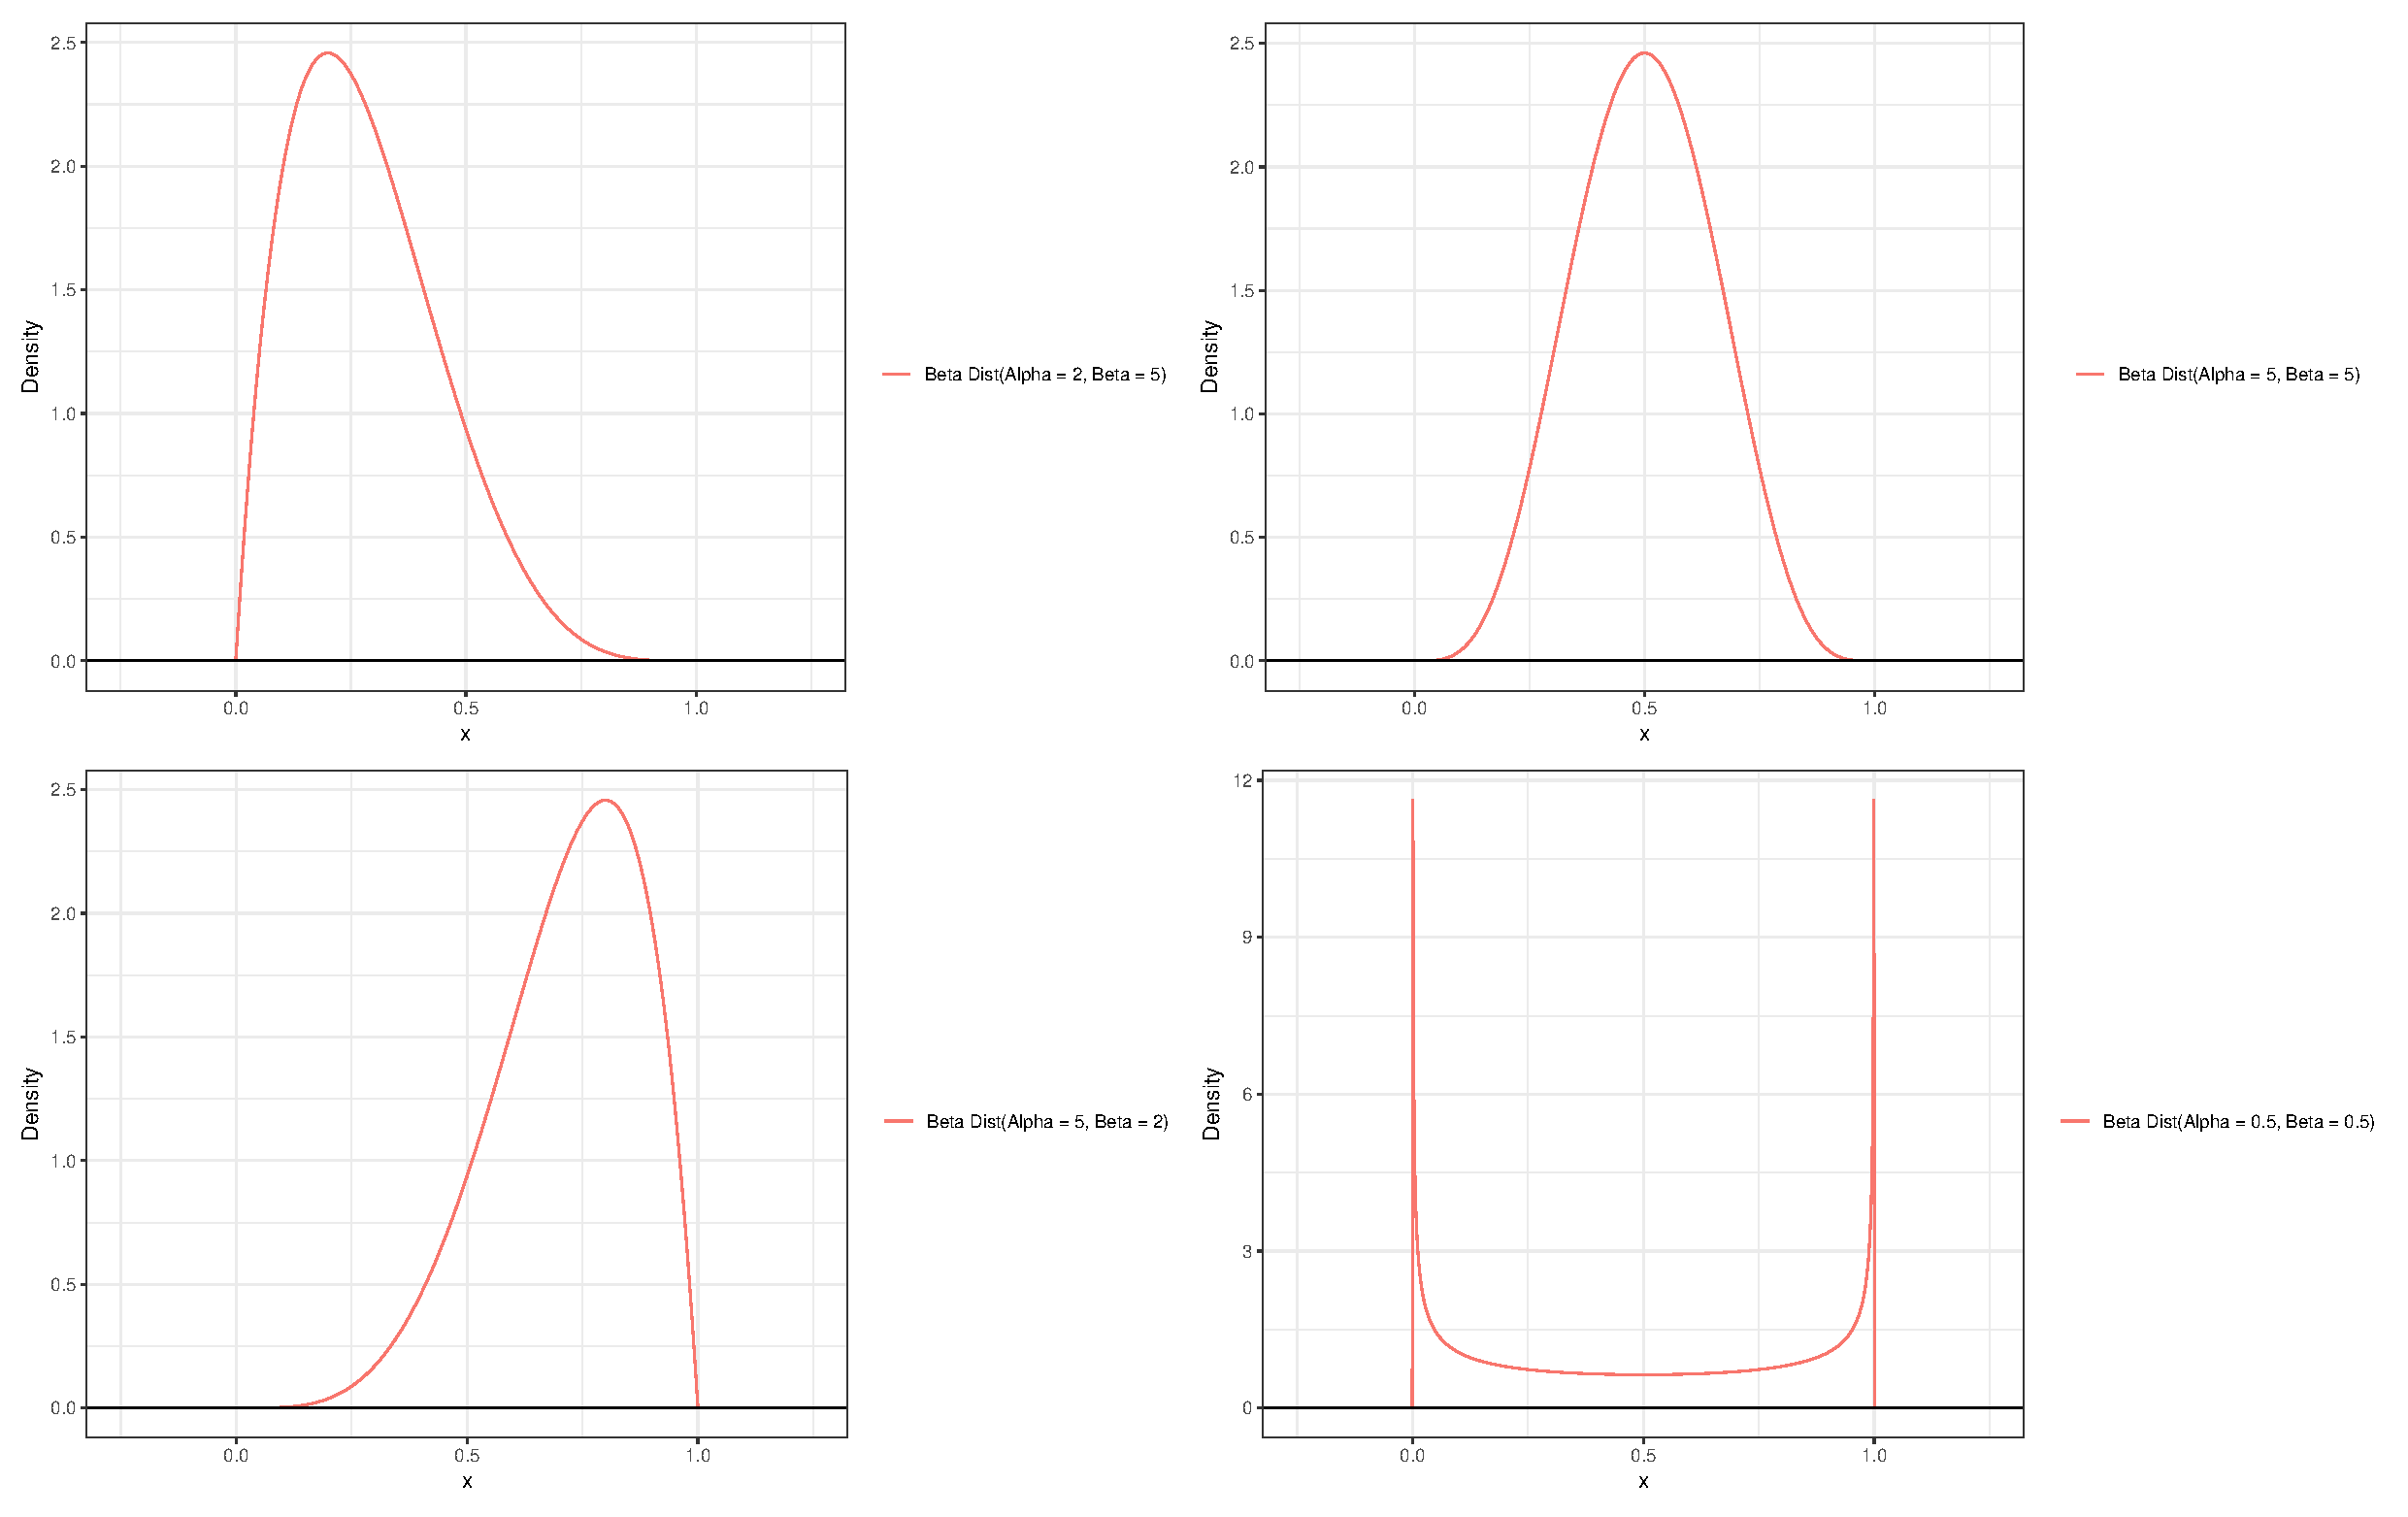
\includegraphics[width=0.9\textwidth]{beta_distributions.pdf}
\caption{Probability Density Functions for Different Beta Distributions}
\end{figure}

\begin{figure}[h]
\centering
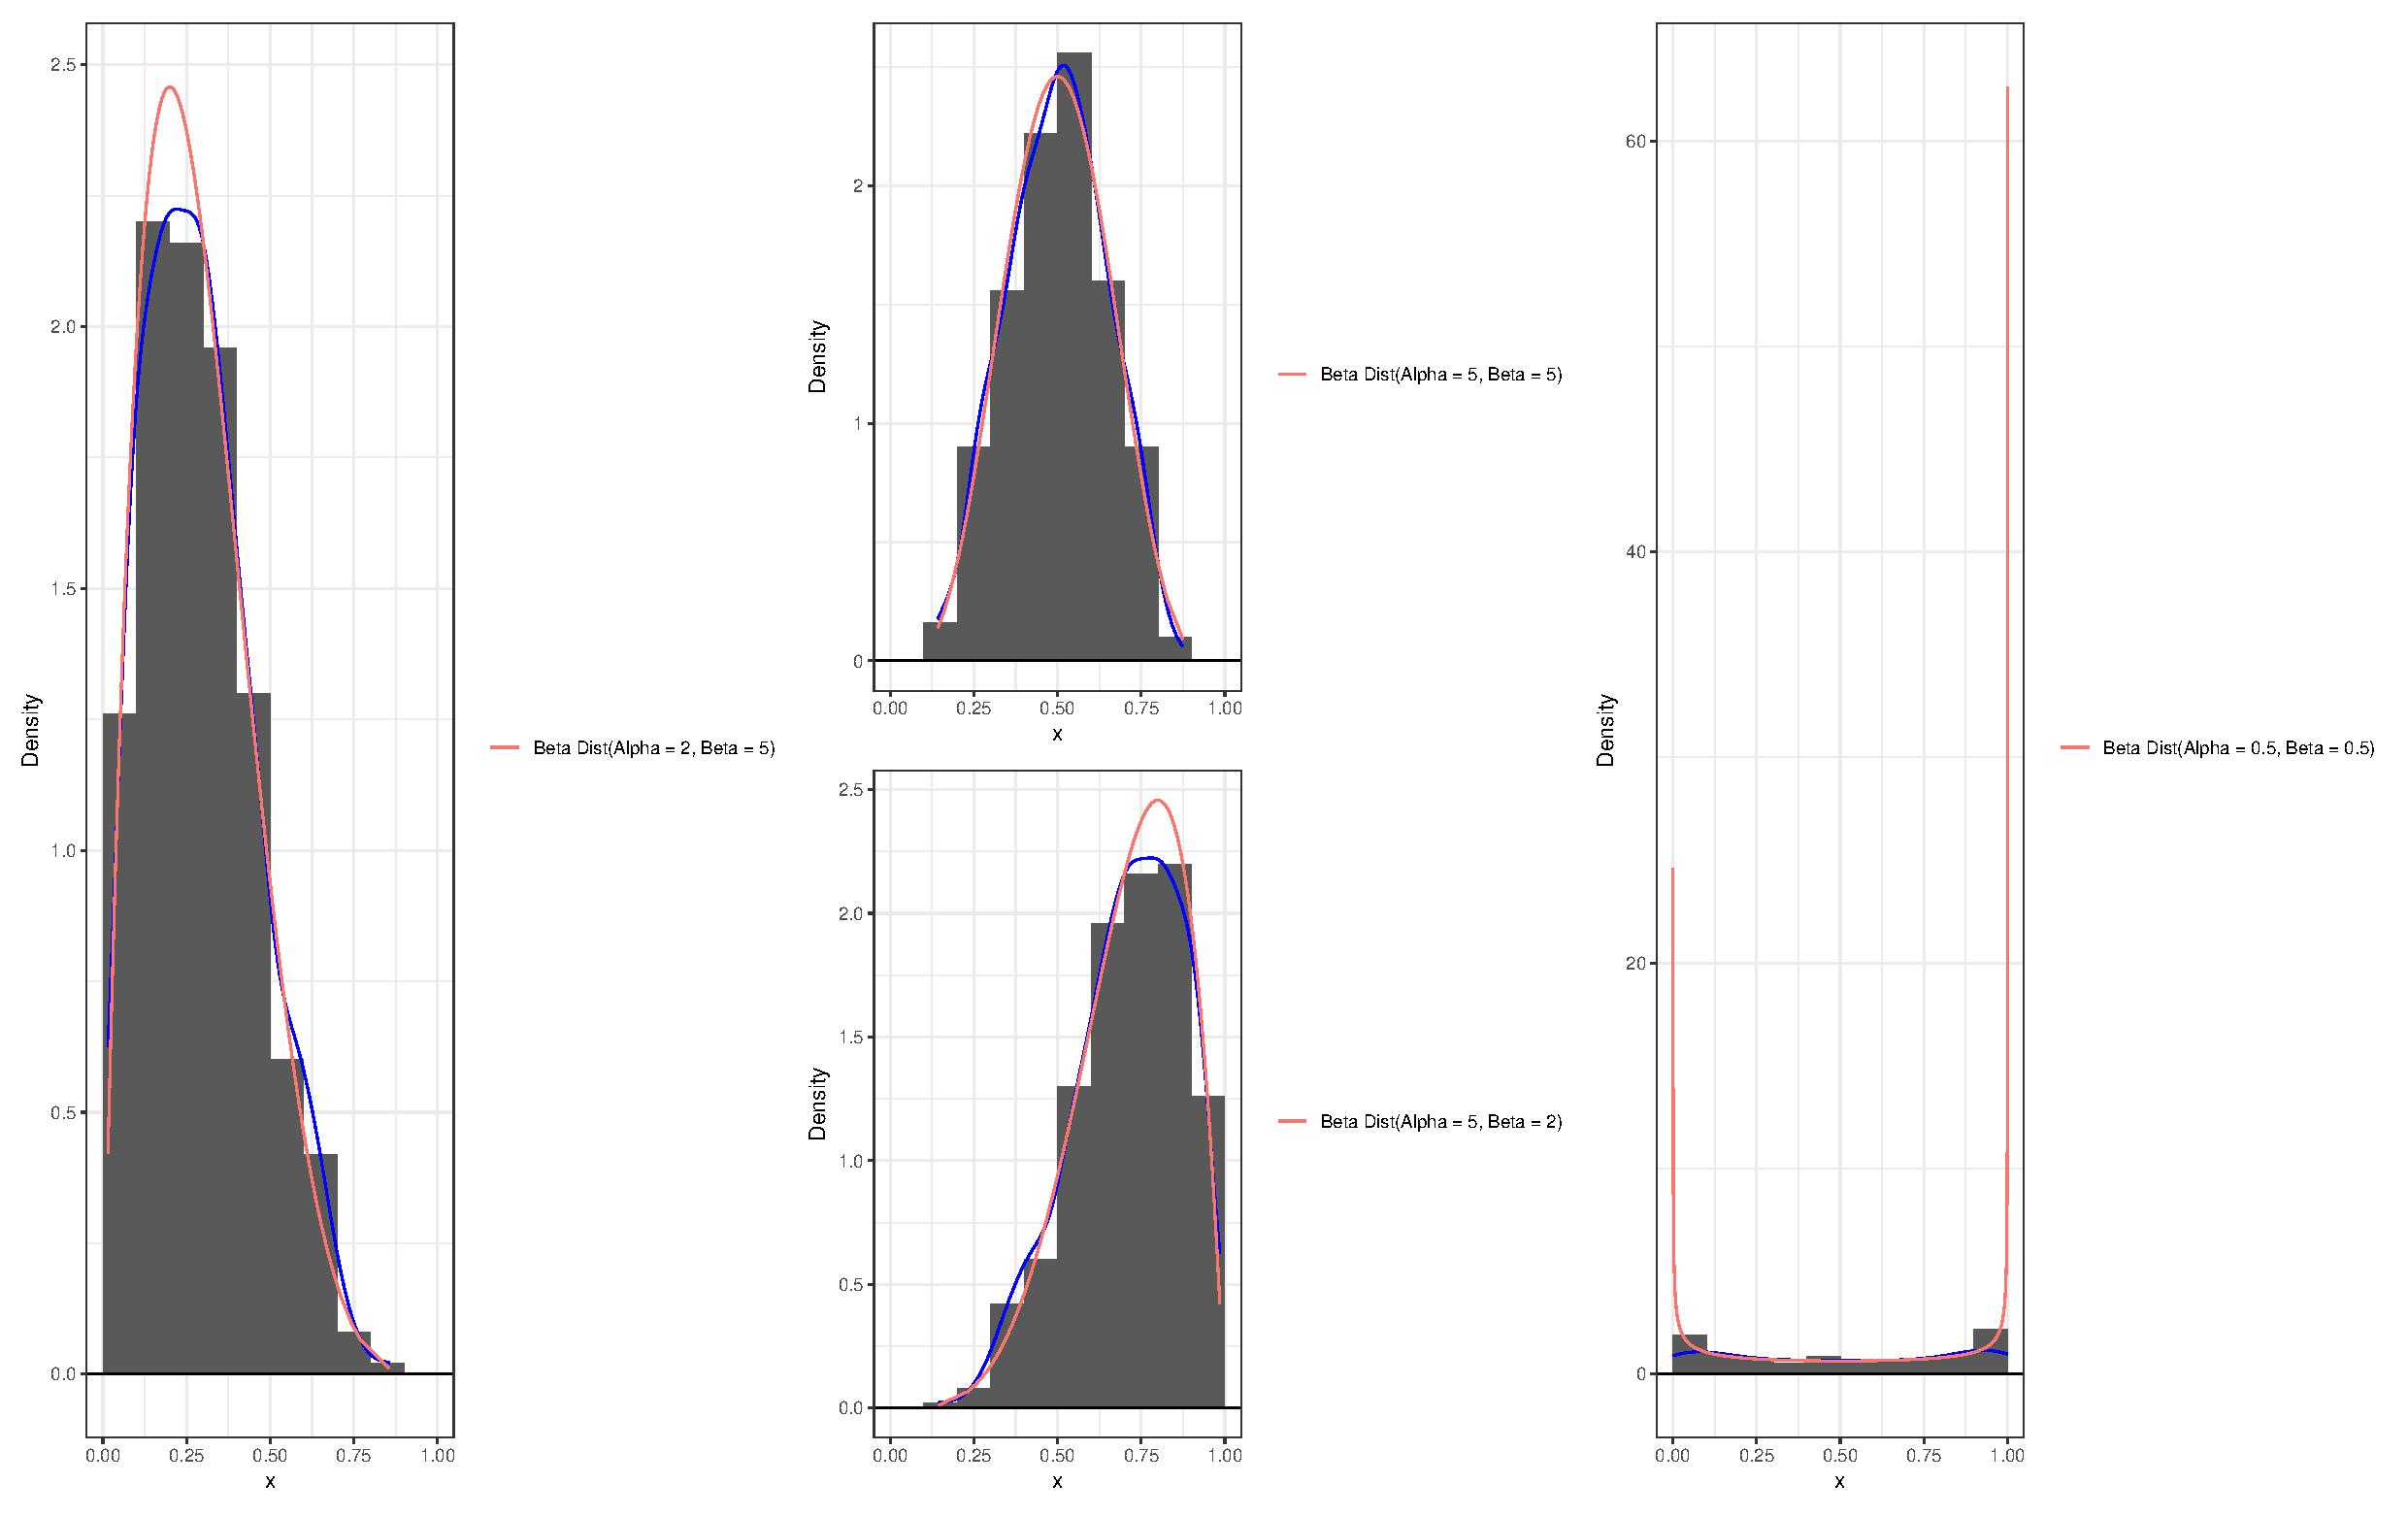
\includegraphics[width=0.9\textwidth]{sample_beta_distributions.pdf}
\caption{Histograms and Estimated Densities from Sample Data Compared to True PDFs}
\end{figure}

\begin{figure}[h]
\centering
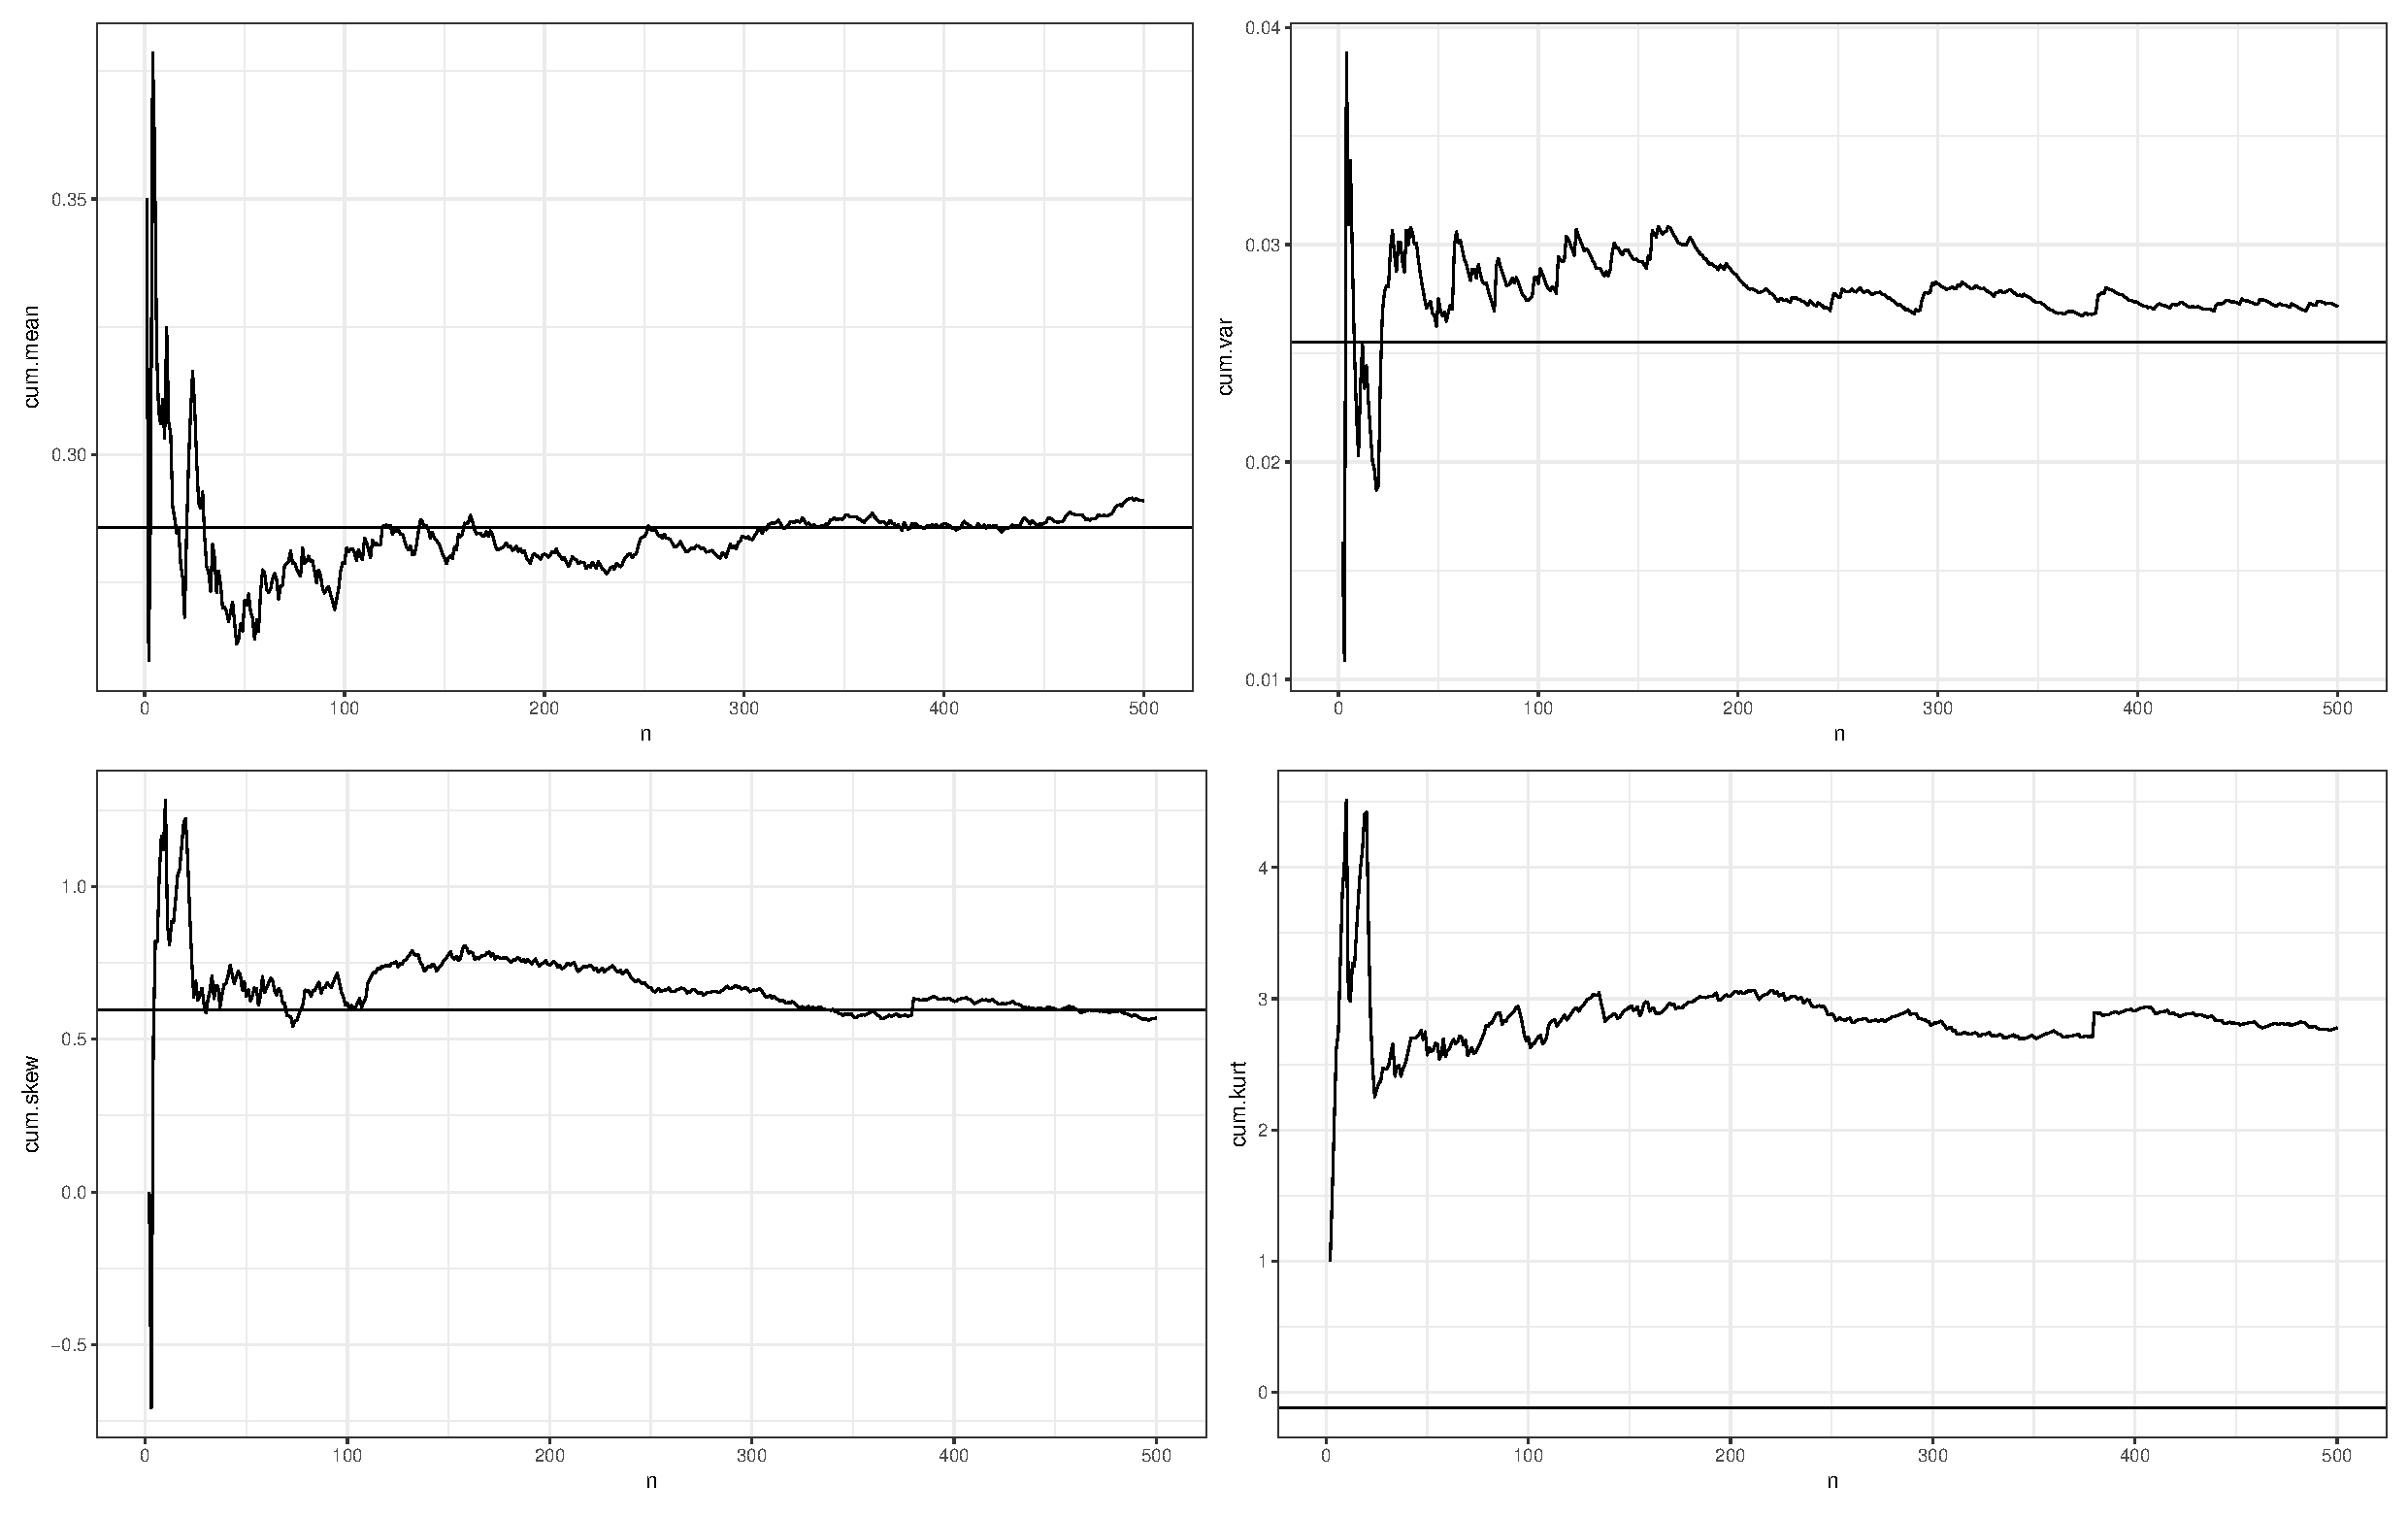
\includegraphics[width=0.9\textwidth]{cum_stats_plots.pdf}
\caption{Cumulative Statistics for Beta(2, 5) Sample}
\end{figure}

\begin{figure}[h]
\centering
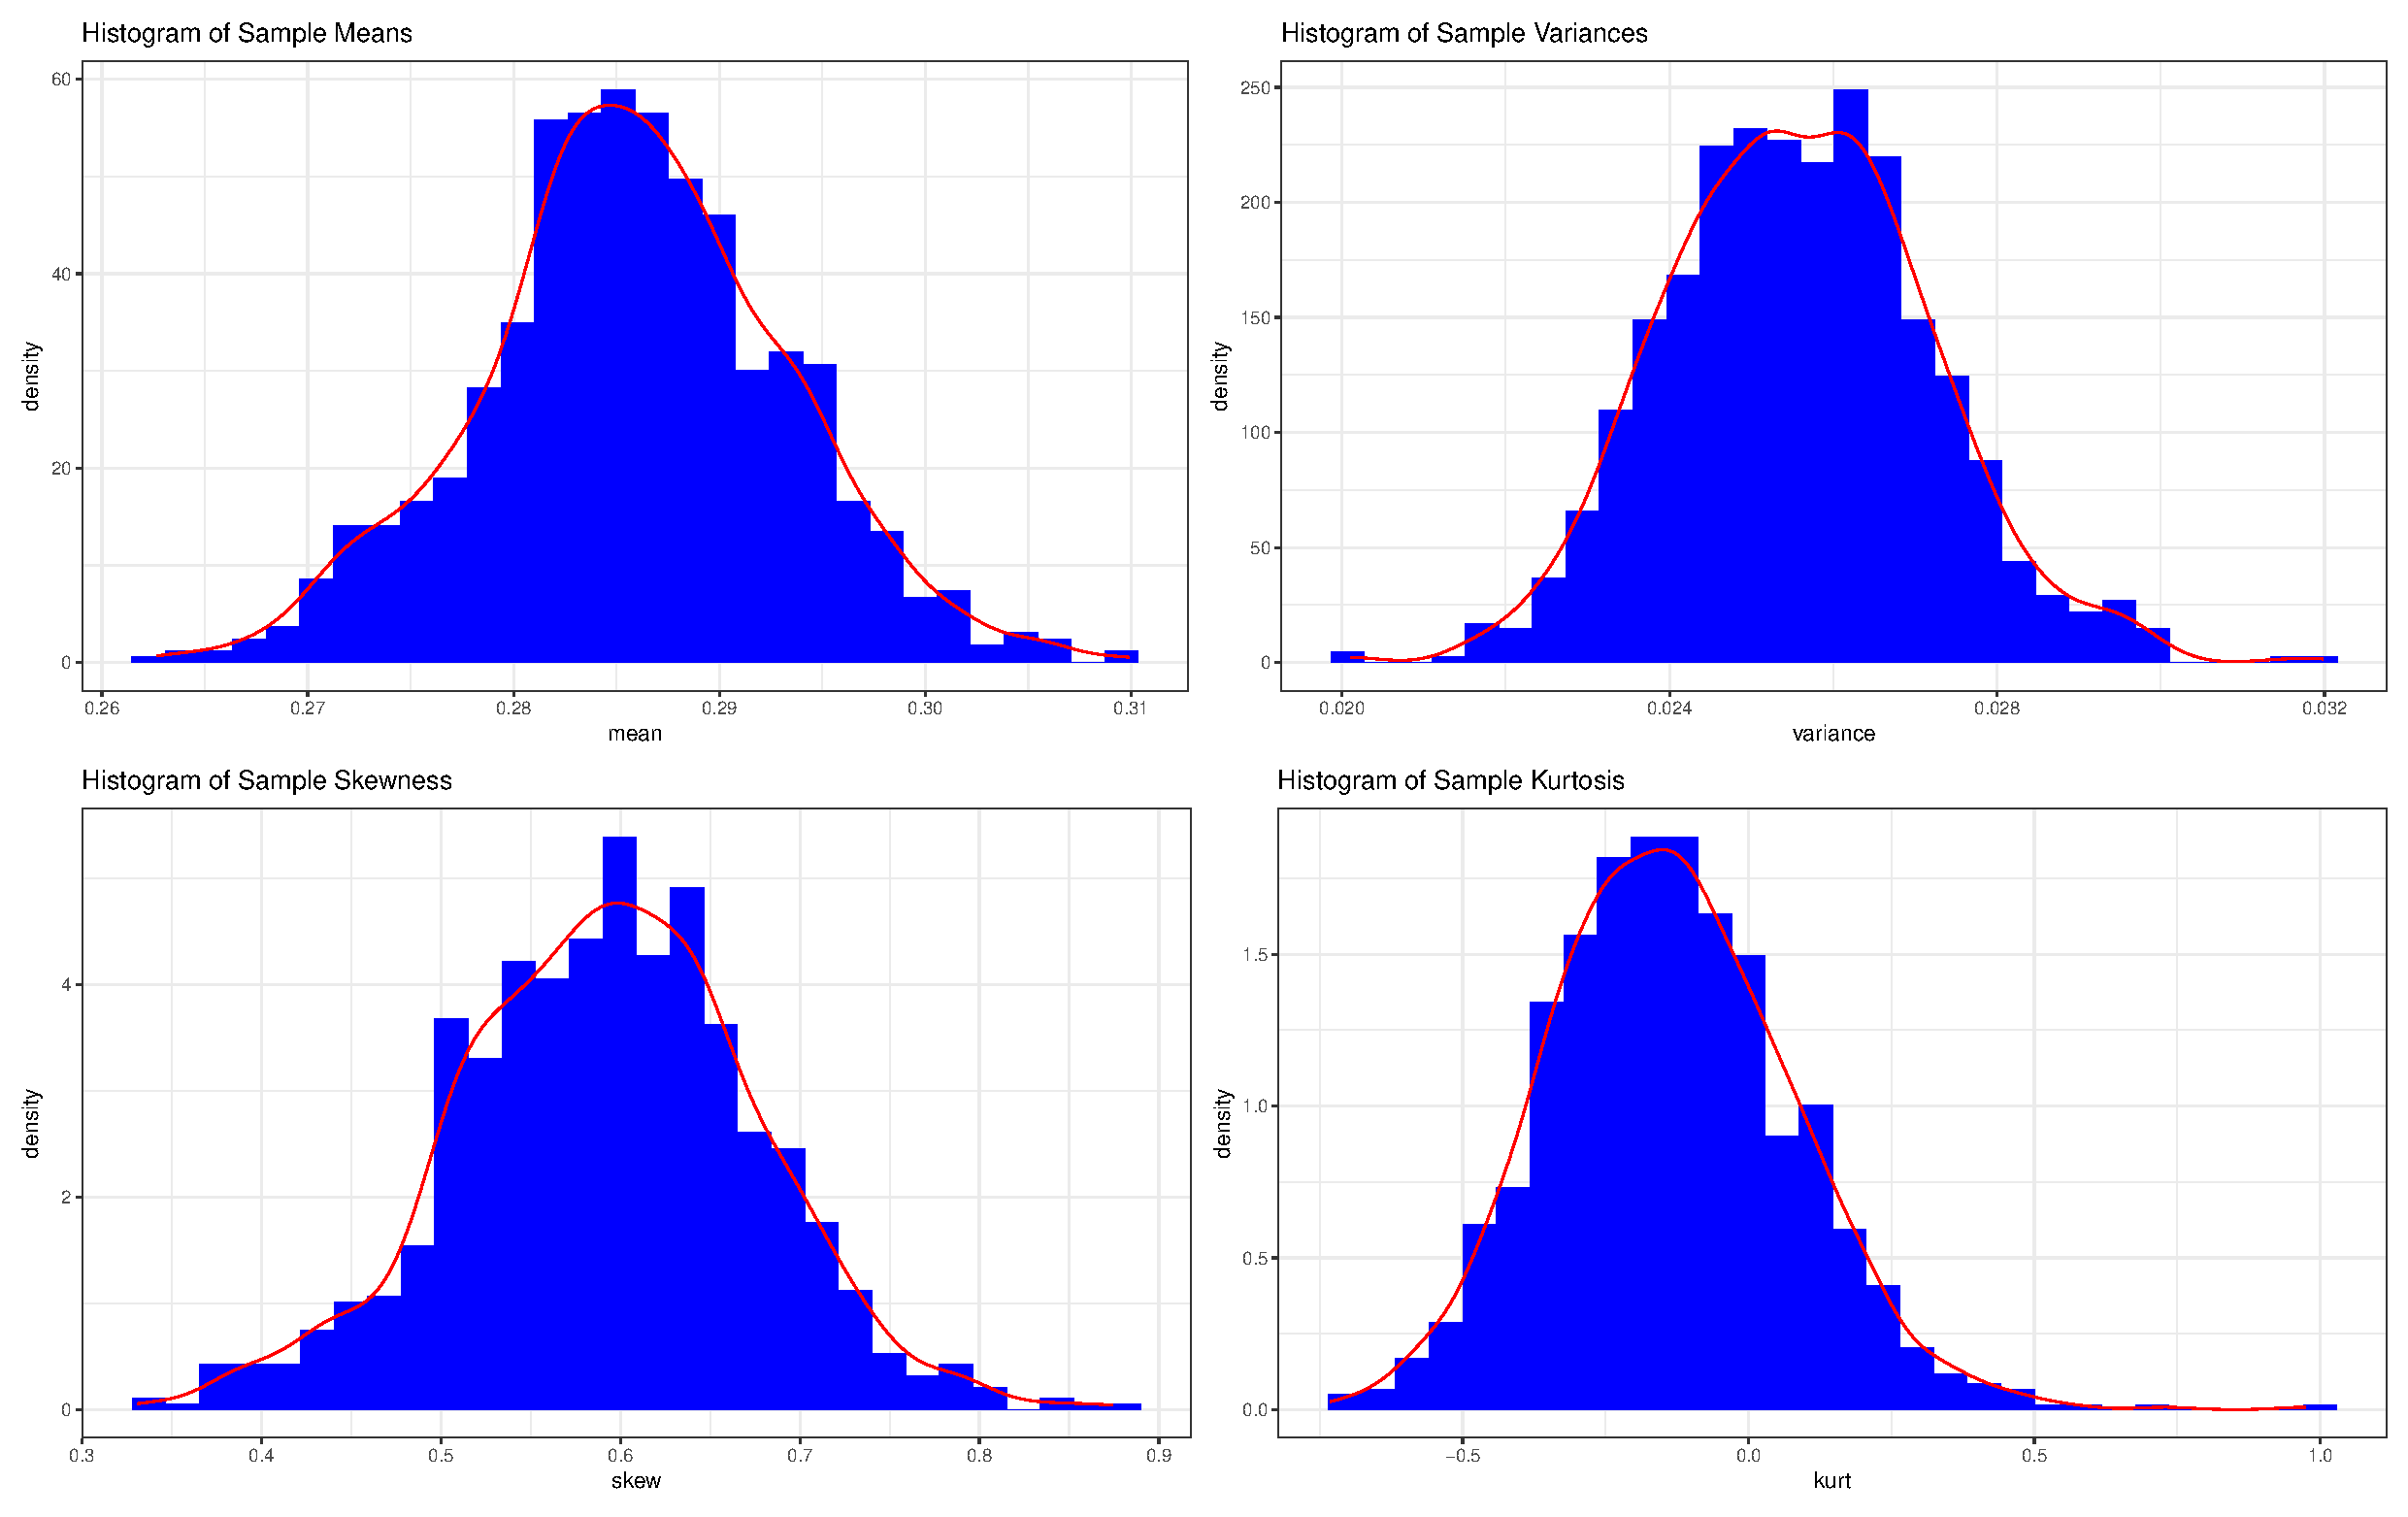
\includegraphics[width=0.9\textwidth]{sample_stats_histograms.pdf}
\caption{Sampling Distributions from 1000 Simulated Samples}
\end{figure}

\begin{figure}[h]
\centering
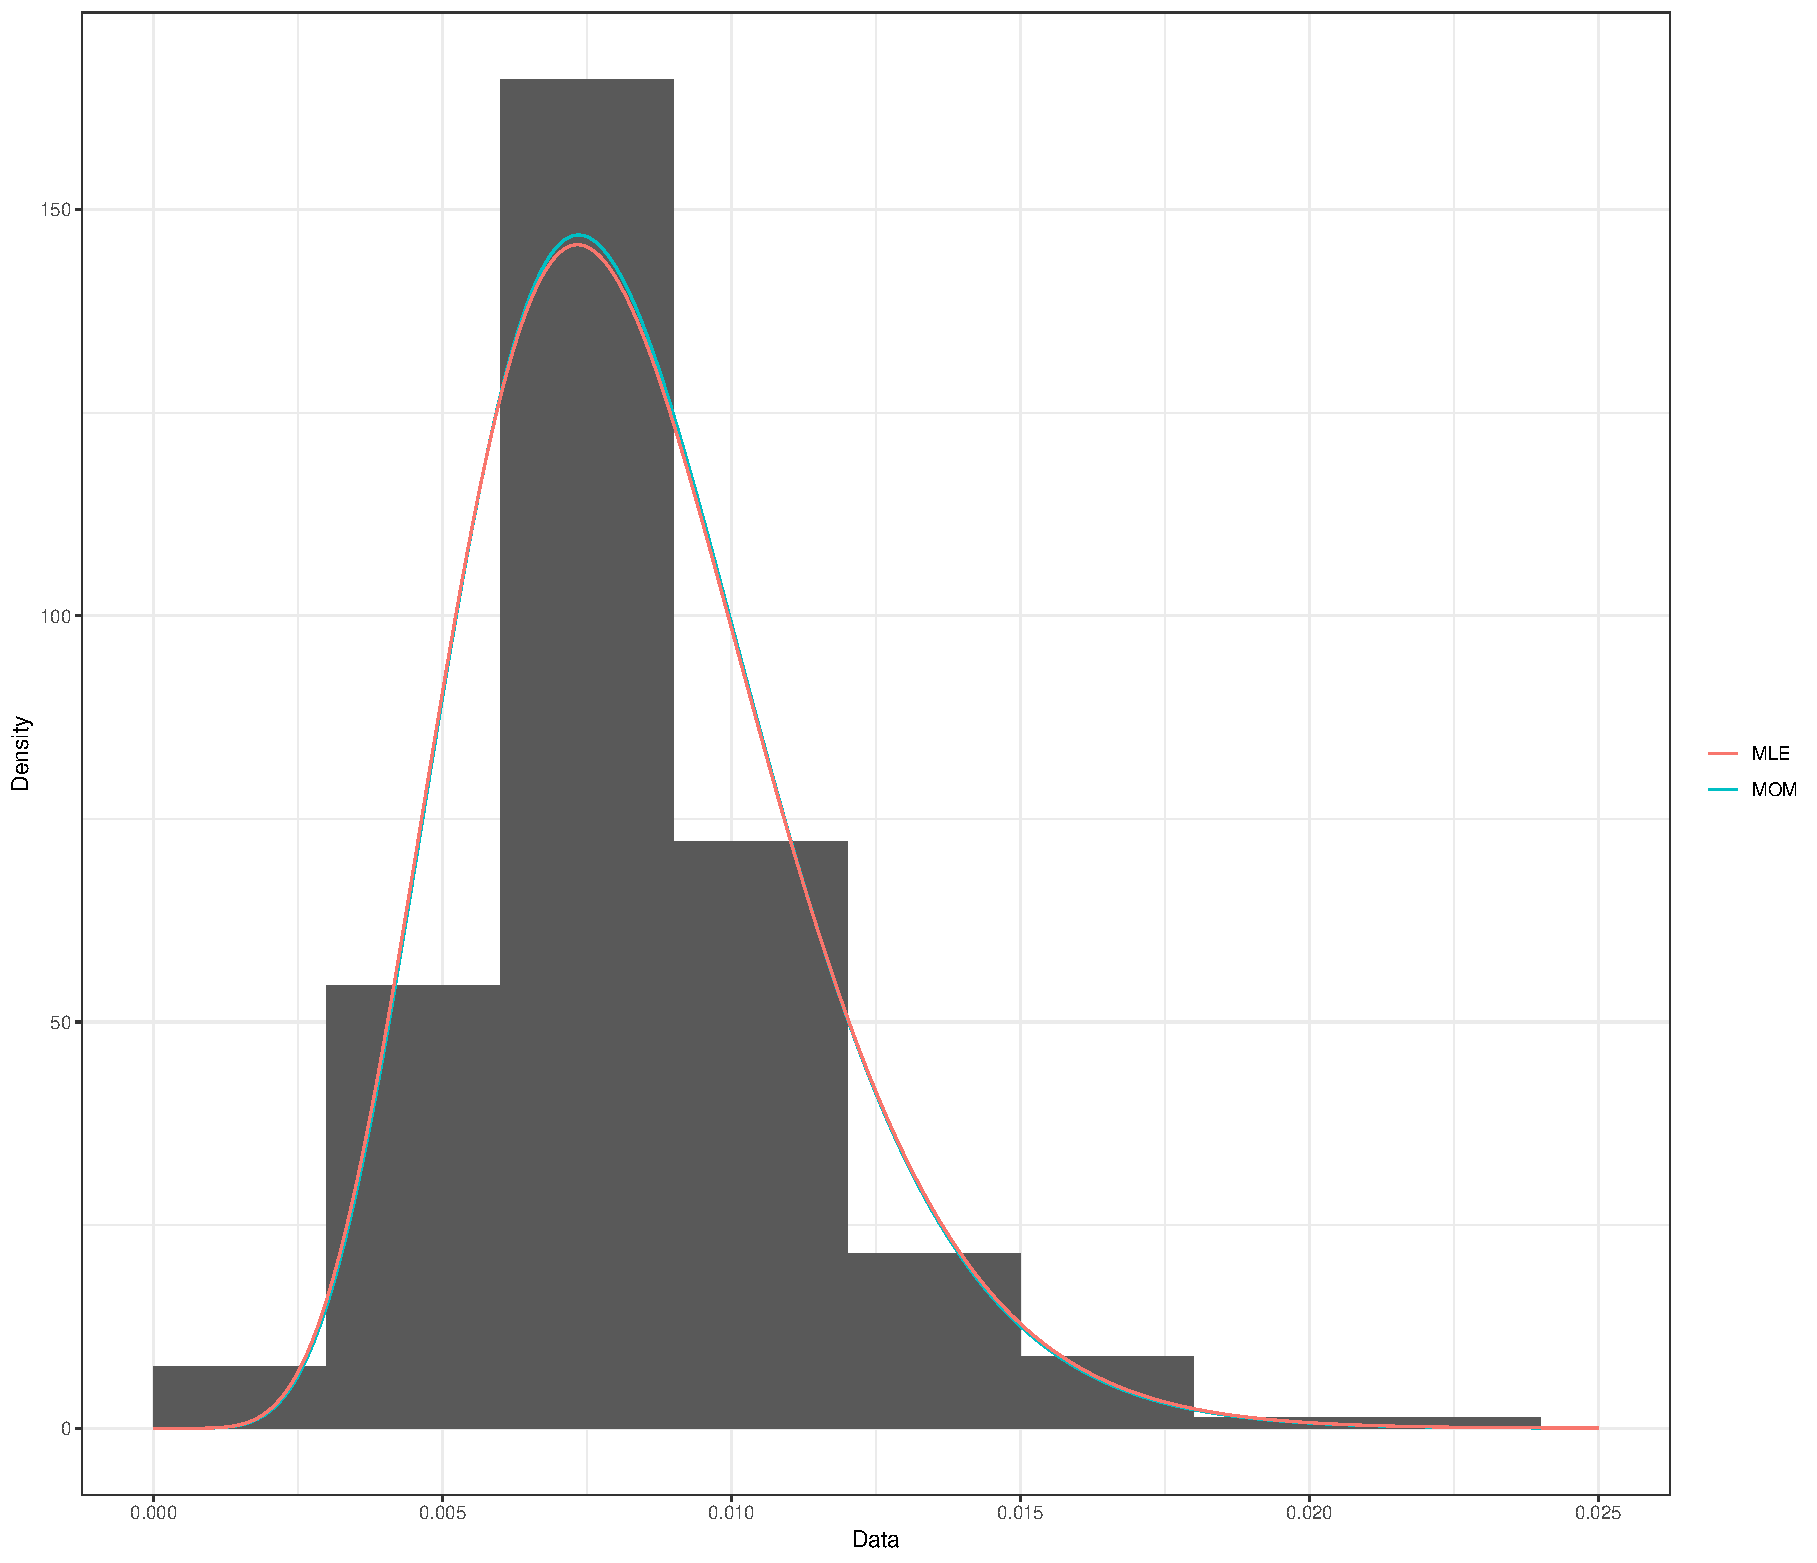
\includegraphics[width=0.7\textwidth]{MOM_MLE_histogram.pdf}
\caption{Histogram of Real Death Rate Data with MOM and MLE Fits}
\end{figure}

\begin{figure}[h]
\centering
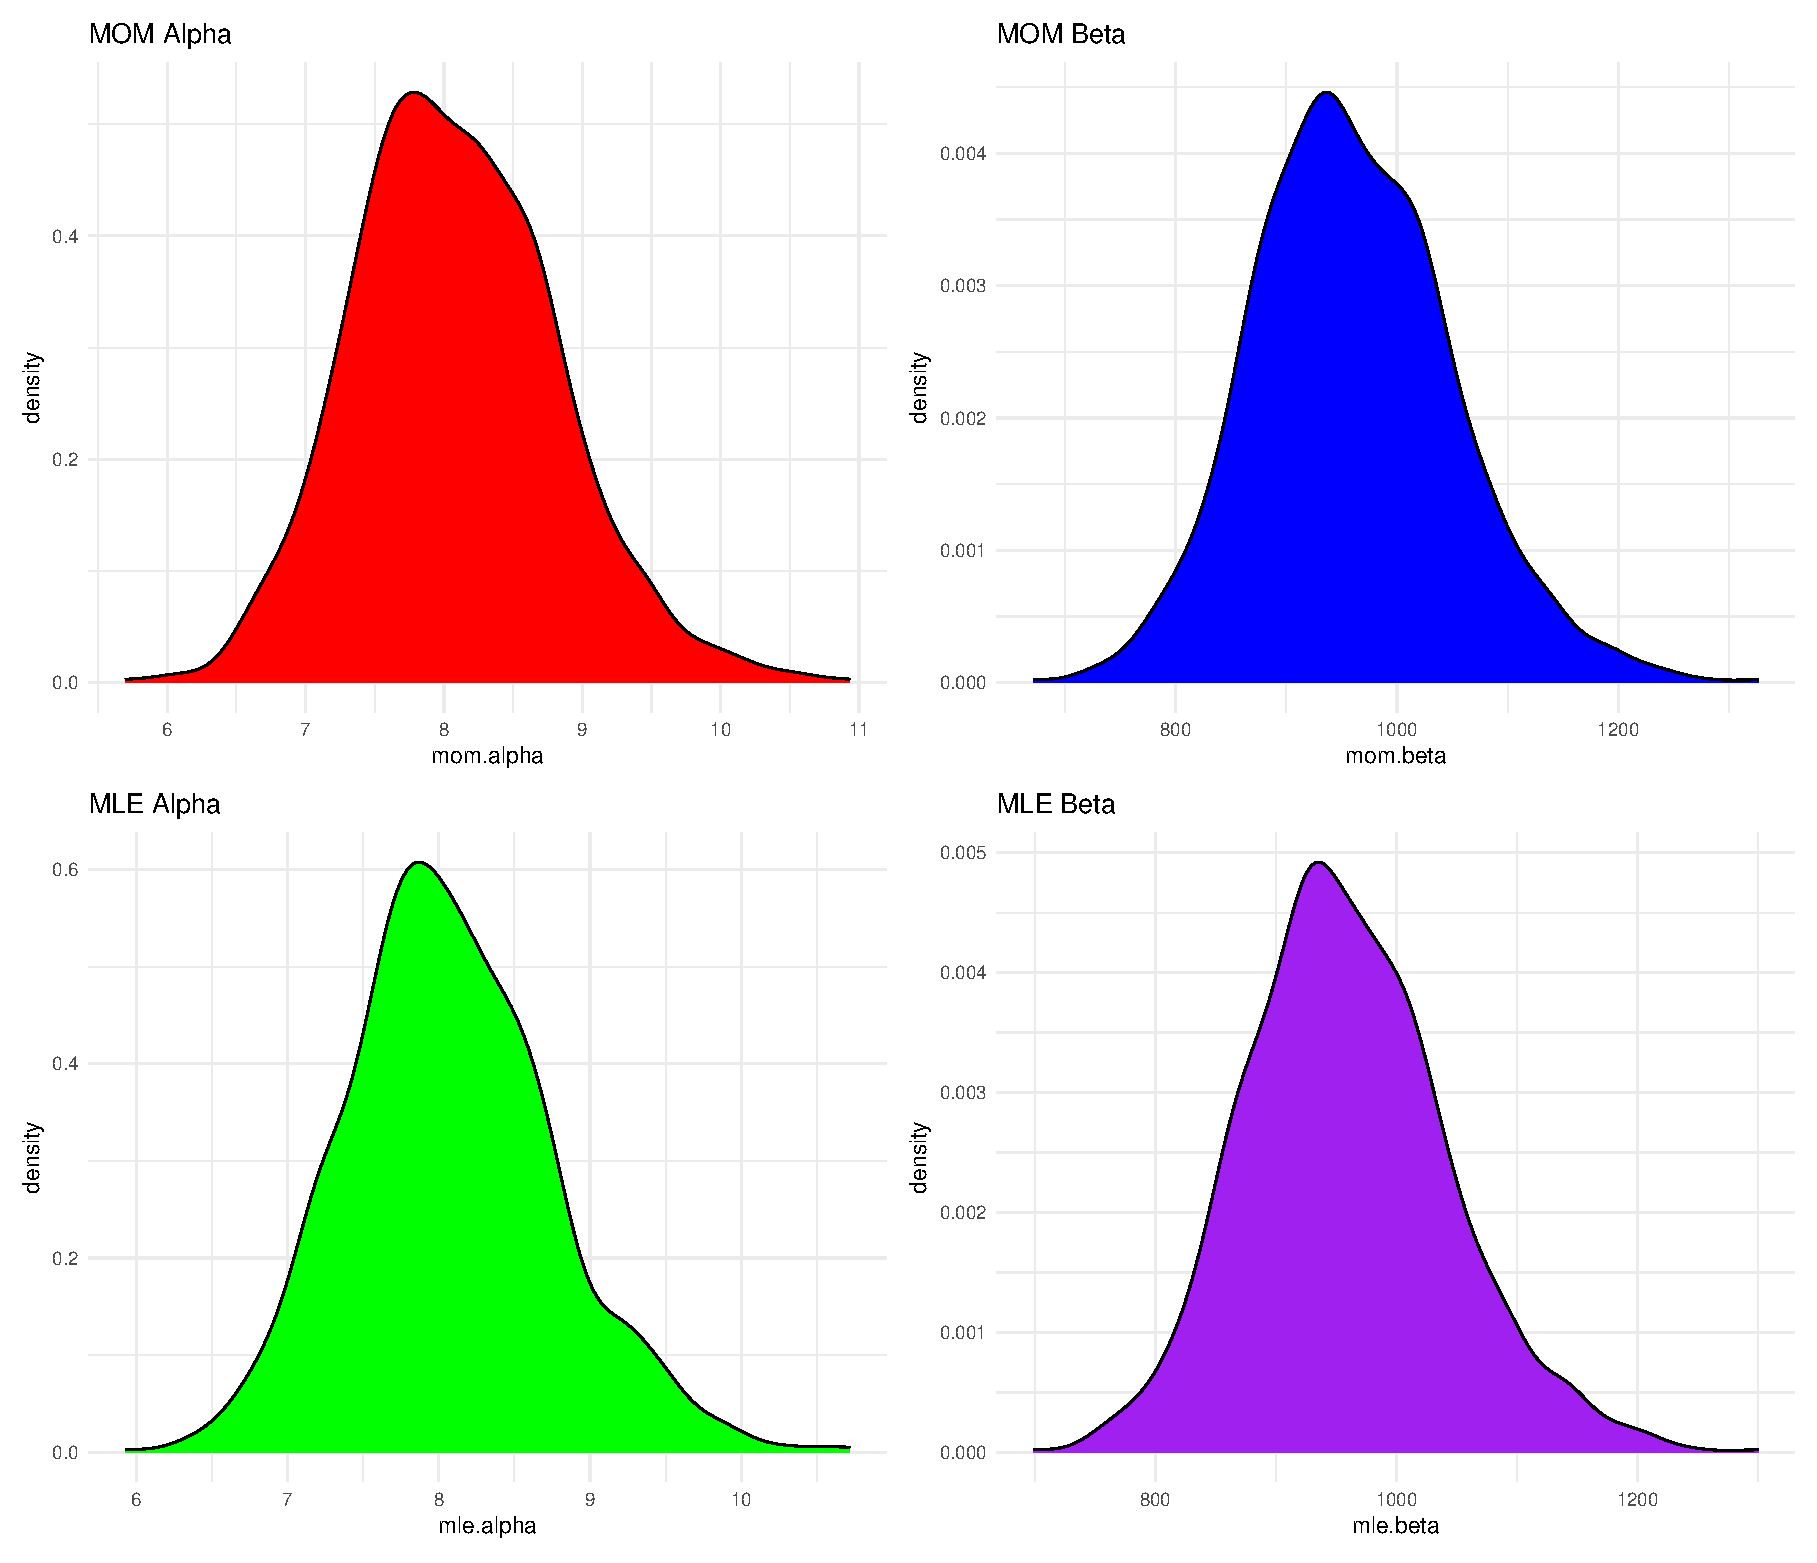
\includegraphics[width=0.9\textwidth]{alpha_beta_densities.pdf}
\caption{Distributions of Estimated $\alpha$ and $\beta$ Values from MOM and MLE}
\end{figure}

\end{document}
